\documentclass[]{thesis-ekf}
\usepackage[T1]{fontenc}
\PassOptionsToPackage{defaults=hu-min}{magyar.ldf}
\usepackage[magyar]{babel}
\usepackage{mathtools,amssymb,amsthm,pdfpages,listingsutf8,hyperref,xurl,xcolor,lmodern,caption,hyperref,longtable,array}


\footnotestyle{rule=fourth}

\newtheorem{tetel}{Tétel}[chapter]
\theoremstyle{definition}
\newtheorem{definicio}[tetel]{Definíció}
\theoremstyle{remark}
\newtheorem{megjegyzes}[tetel]{Megjegyzés}

\renewcommand{\lstlistingname}{kód}
\lstdefinestyle{user1}{
	inputencoding=utf8/latin2,
	basicstyle=\footnotesize\ttfamily,
	columns=fullflexible,
	numbers=left,
	breaklines,
	xleftmargin=1cm,
	xrightmargin=1cm,
	postbreak=\hbox{$\color{red}\hookrightarrow$\ },
	backgroundcolor=\color{gray!10},
	frame=tblr,
	framesep=2pt,
	keywordstyle=\bfseries\color{blue},
	commentstyle=\itshape\color{red},
}
\lstdefinelanguage{JavaScript}{
	keywords={cy, get, contains, describe, it, select, type, click, const, attachFile, next, location, should, visit},
}
\lstdefinelanguage{PHPOwn}{
	keywords={use, return, new, class, extends, public, void, function, Schema, create, id, unsignedBigInteger, string, integer, text, nullable, timestamps, foreign, references, on, cascade, down,dropIfExists, @extends, @section, @foreach, @endforeach, @if, @else, @endif, {{, }}, asset, @endsection, th, td, div, tr, table, protected, \$table, \$primaryKey, \$fillable, \$this, hasMany, belongsTo, redirect, route, with, compact, view, namespace, if, find, \$advertisement, Advertisement, Route, get, require, name, mobile_number, user, description, price, category, city, county, title},
	morecomment=[l]{//},
	morecomment=[s]{/*}{*/},
	morestring=[b]',
	morestring=[b]",
	sensitive=true,
}


\begin{document}
	\institute{Matematikai és Informatikai Intézet}
	\title{Adatbázis alapú web alkalmazás fejlesztése}
	\author{Verebélyi Valentin\\Programtervező Informatikus BSc}
	\supervisor{Dr.~Tajti Tibor Gábor\\Egyetemi Docens}
	\city{Eger}
	\date{2024}
	\maketitle
	\tableofcontents
	
	\chapter*{Bevezetés}
	\addcontentsline{toc}{chapter}{Bevezetés}
	\begin{center}
		\url{https://github.com/rcfr84/Szakdolgozat}
	\end{center}
	Én abból az indíttatásból választottam az adatbázis alapú webalkalmazás projektet, mivel hozzám közel állnak a webes alkalmazások. Maga a projekt témája az nem más, mint egy apróhirdetés weboldal. Azért választottam ezt a projekt ötletet, mivel nagyon érdekesnek találtam, illetve kellő bonyolultságúnak tartottam egy szakdolgozati projekthez. Ezen kívül pedig az én véleményem szerint van aktualitása a projektemnek, mivel Magyarországon jelenleg nem lenne sok konkurenciája, illetve a tapasztalatom szerint sokan élnek az ilyenféle rendszerek használatával manapság. Fontosnak tartom megemlíteni, hogy ezt az alkalmazást a kezdetektől fogva a Magyarország területén élők számára terveztem megvalósítani. Az volt a célom az alkalmazásommal létrehozásával kapcsolatban, hogy belelássak egy ilyen komplex alkalmazás elkészítésébe, felépítésébe és ezeknek köszönhetően a szerzett tapasztalatok által bővítsem a tudásomat, tapasztalatomat a webes projektek területén és a jövőben ezek a tapasztalatok a hasznomra fognak válni. Az elkövetkezendő néhány fejezeteben szeretném Önnek bemutatni és ismertetni az általam készített adatbázis alapú webalkalmazásomat. Először majd magáról az alkalmazásom tervezéséről lesz szó, röviden érinteni fogom a tervezéshez kötődő, általam hasznosnak vélt információkat. Ezt követően pedig a fejlesztésről teszek majd meg néhány említést, azonban ebben a fejezetben főként a fejlesztéshez használt eszközök és technológiák bemutatásáról fog szólni. Ezek után pedig a tesztelésről ejtek majd meg pár gondolatot, megosztok Önnel különböző tesztelési technikákat és röviden ismertetni is fogom őket. A célom, ezzel a fejezettel, hogy egy átfogó képet adjak magáról a tesztelésről, illetve a fontosságáról is. Az utolsó előtti fejezetben részletesen bemutatom az adatbázis alapú webalkalmazásomban megvalósított különböző jogosultságokkal rendelkező felhasználók által elérhető funkciókat. Végül pedig az utolsó fejezetben alaposan tárgyalom majd meg, hogy hogyan épül fel az alapoktól a megvalósításig egy a projektemben szereplő nézet és annak a hozzá tartozó funkciói. A könnyebb és átláthatóbb megértés érdekében, valamint a szakdolgozat illusztrálása céljából néhány ábrát és képet fogok használni az alkalmazásom egyes funkcióinak bemutatásához, illetve néhány kódrészletet is szeretnék bemutatni majd Önnek. Összességében tehát, az adatbázis alapú webalkalmazás projekt választása nemcsak az érdeklődésemet tükrözi a webfejlesztés iránt, hanem lehetőséget kínál számomra arra is, hogy elmélyedjek egy izgalmas és változatos témában, és fejlesszem a tudásomat, illetve a tapasztalataimat is. Bízom benne, hogy sikerült felkeltenem az Ön érdeklődését a választott témával kapcsolatban. 
	
	\chapter{Tervezés}
		A tervezés egy nagyon fontos, központi szerepet tölt be egy szoftvereknél. Az én meglátásom és tudásom szerint a következő okok miatt szükséges tervezni:
		\begin{enumerate}
			\item Tervezési célok meghatározása: fontos az, hogy mind a fejlesztő, mind a megrendelő egyértelműen megértse, hogy pontosan mit kell elérni a szoftverrel.
			\item Költség- és időmegtakarítás: implementálás előtt, ha kellő alapossággal tervezzük meg a szoftvert, akkor segíthet kiszűrni a későbbi fázisokban esetleges előforduló hibákat. 
			\item Bővíthetőség: ez alatt azt értem, hogy a szoftver úgy kell megtervezni, hogy fel legyen készítve arra, hogy lehessen hozzáadni könnyedén új funkciókat.
			\item Funkciók és feladatok felosztása: ez azért lehet hasznos, mivel a fejlesztés során a fejlesztők pontosan csak az ő általuk elvállalt feladatokat valósítják meg.
			\item Kommunikáció segítése: ha van egy jól kidolgozott terv, akkor ha a fejlesztők elakadnak valamiben vagy nem értik meg pontosan, hogy mit és hogyan kell implementálni, akkor elég, ha megnézik a tervben az adott dologhoz kapcsolódó részeket és ezáltal megtudják oldani a rájuk bízott feladatot.
		\end{enumerate}
		Azonban az imént felsoroltakon kívül még számtalan okok miatt szükséges a tervezni. A következőben az én általam készített adatbázis alapú webalkalmazásomnak a követelménylistája látható. A követelménylistában azokat a funkciókat szükséges dokumentálni, amikkel a programoknak rendelkeznie kell. Ez általában a különböző projektek esetében a követelmény specifikációban található meg. A követelmény specifikáció egy olyan dokumentáció, amelyben az igények, követelmények kerülnek meghatározásra, ennek az alapja a riportok. A riportok segítségével lehetséges felmérni a megrendelő követelményeit. \Aref{kovetelmenylista}.~táblázatban megtekinthető a projektem követelmény listája, ami \aref{ch-fugg}.~fejezetben található meg.
		
	\section{A tervezéshez alkalmazott eszközök és technológiák}
		A következő alszakaszokban a tervezéshez használt eszközökről és technológiákról lesz majd szó, melyeknek bemutatásaival az a célom, hogy alaposabb megértést nyújtsak az adatbázis alapú webalkalmazásomhoz kapcsoló alkalmazott eszközökről és technológiákról.
	\subsection{DBDiagram}
	A dbdiagram segítségével van lehetőség arra, hogy egy alkalmazás adatbázisának a sémáját és struktúráját megtervezzük, és ehhez ad egy vizuális képet számunkra. A DBML-t, azaz Database Markup Language használja, amit magyarul talán adatbázis jelölőnyelvként tudnék lefordítani. Amiért a véleményem szerint nagyon hasznos még az nem más, mint, hogy rengetegféle olyan opciót ad számunkra, amire szükségünk lehet. Ilyen opciók például azok, hogy van lehetőség importálni be kódot MySQL, PostgreSQL\footnote{Ez nem más, mint gy relációsadatbázis-kezelő rendszer}, Rails\footnote{Ez egy keretrendszer webalkalmazások készítéséhez.} valamint SQL szerverről. Ugyanezeket a típusú kódokat kilehet exportálni az imént megemlített típusokba, kivéve a Rails, mivel oda nem lehetséges. Ezenkívül van még olyan opció is, hogy ki lehet exportálni PNG, SVG\footnote{XML alapú leírónyelv.} vagy akár PDF formátumba is az elkészült tervet. A dbdiagram alap változata ingyenesen használható mindenki számára. \cite{Dbdiagram}
	
	\begin{figure}[ht!]
		\centering
		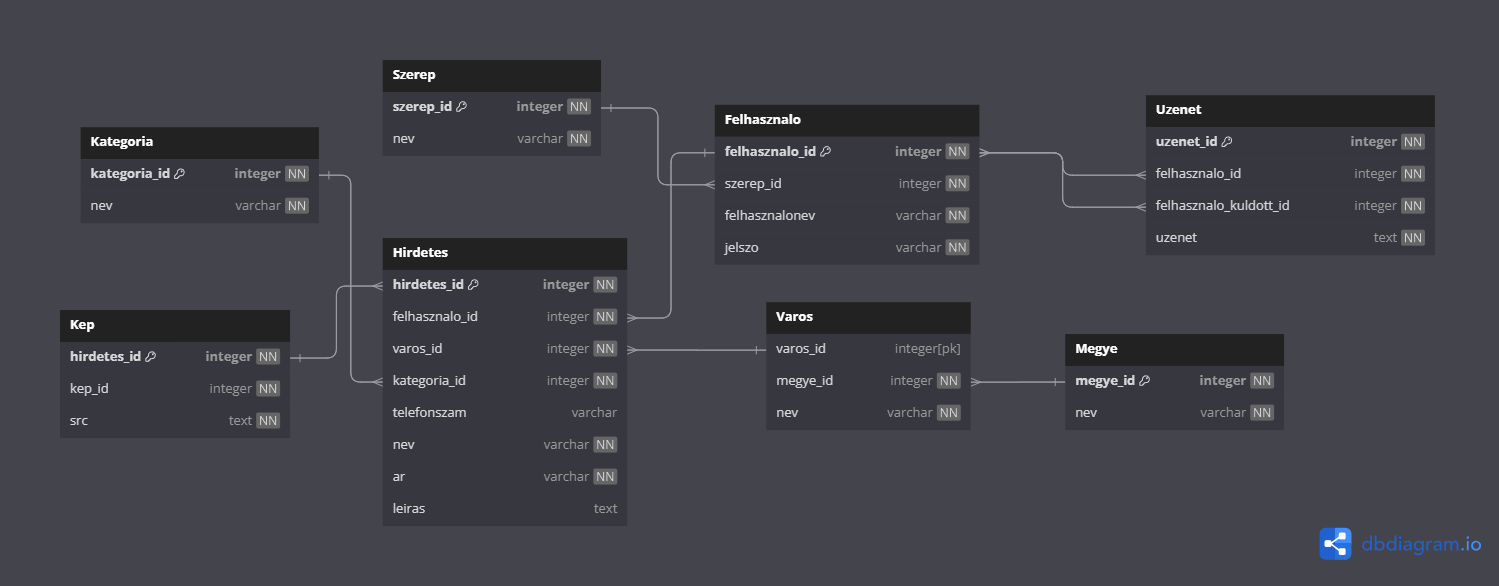
\includegraphics[width=15cm]{./tervezes/dbdiagram}
		\caption{Adatbázisterv (Saját készítés)} 
		\label{dbdiagram}
	\end{figure}
	
	A következőkben \aref{dbdiagram}.~képen látható adatbázistervről szeretnék egy pár gondolatot megosztani. Pontosabban arról, hogy hogyan milyen táblákból áll és milyen kapcsolatok találhatóak meg táblák között. Látható, hogy ez a véleményem szerint egy közepes mennyiségű táblából álló adatbázisterv. Kezdjük a felhasználó nevű táblával, ahogyan, mint minden sok más hasonló webalkalmazás esetén itt is szükséges eltárolni egy email címet, egy felhasználónevet, illetve egy jelszót. Ezeken kívül egy másik táblából, nevezetesen a szerep nevű táblából pedig kap egy a megfelelő jogosultság ellenőrzéséhez egy azonosítót. Itt a két tábla között egy-a-többhöz kapcsolat áll fent, mivel egy szerepel rendelkező felhasználóból több is lehetséges. Ez a kapcsolat több helyen is előfordul még az adatbázistervemben, például a város és vármegye tábla között is fennáll. Látható még egy üzenetek tábla is, amivel két felhasználó képes szöveges üzeneteket küldeni egymásnak. Itt a két tábla között már a több-a-többhöz kapcsolat áll fenn, mivel egy felhasználó több üzenetet küldhet vagy kaphat, tehát egy felhasználóhoz több üzenet is tartozhat. Utolsóként pedig a hirdetés tábláról szeretném megosztani a gondolataimat. A meglátásom szerint egy hirdetés eltárolásához egy hirdetésnév, egy ár, egy leírás, egy kategória név, egy város név és egy telefonszám mezők megadása nélkülözhetetlen. Ezek a mezők közül csak és kizárólag a telefonszám megadása nem kötelező. 
	
	\subsection{PlantUML}\label{sc-plantuml}
	Az UML a Unified Modeling Language rövidítése, azaz Egységes Modellezési Nyelv. Az UML arra jó, hogy szoftvert tervezzünk vele, a gondolatainkat letudjuk vele rajzolni, skiccelni. Ezenkívül a kiforrott megoldások dokumentálására is használható. A PlantUML egy komponens, aminek a segítségével gyorsan tudunk létrehozni szekvencia-, használati eset- és osztálydiagramokat. Ezenkívül még rengetegféle diagramot tudunk készíteni. \cite{PlantUML}
	
	Manapság a tervezés az használati eset központú. A következő pár mondatban az ilyenféle alapú tervezésről lesz szó. Tulajdonképpen itt azt a kérdést tehetjük fel, hogy ki (angolul: actor) mire (funkció) tudja használni az adott informatika rendszert. Az actor-ról azt érdemes tudni, hogy ő nem része az informatikai rendszernek, hanem ő csak használja azt. Az actor gyakran lehet ember, AI vagy akár egy másik informatikai rendszer. Fontos az is, hogy minden ábra, amit készítünk az visszavezethető legyen a már meghatározott követelmények szintjéig. Az használati alapú tervezés előnye az, hogy egyszerűen, érthetően írja le a rendszer funkcióit. Ebből kifolyólag, mind a megrendelő, mind a tervező számára könnyen érthető az ábra. Tulajdonképpen a használati eset alapú tervezés nem más, mint egy közös nyelv a megrendelő és a tervező között, amit mind a két fél ért.\cite{Kusper Informatikai} \Aref{useCase}.~képen látható a plantUML-ben készített használati eset ábra az alkalmazásomhoz.
	\begin{figure}[ht!]
		\centering
		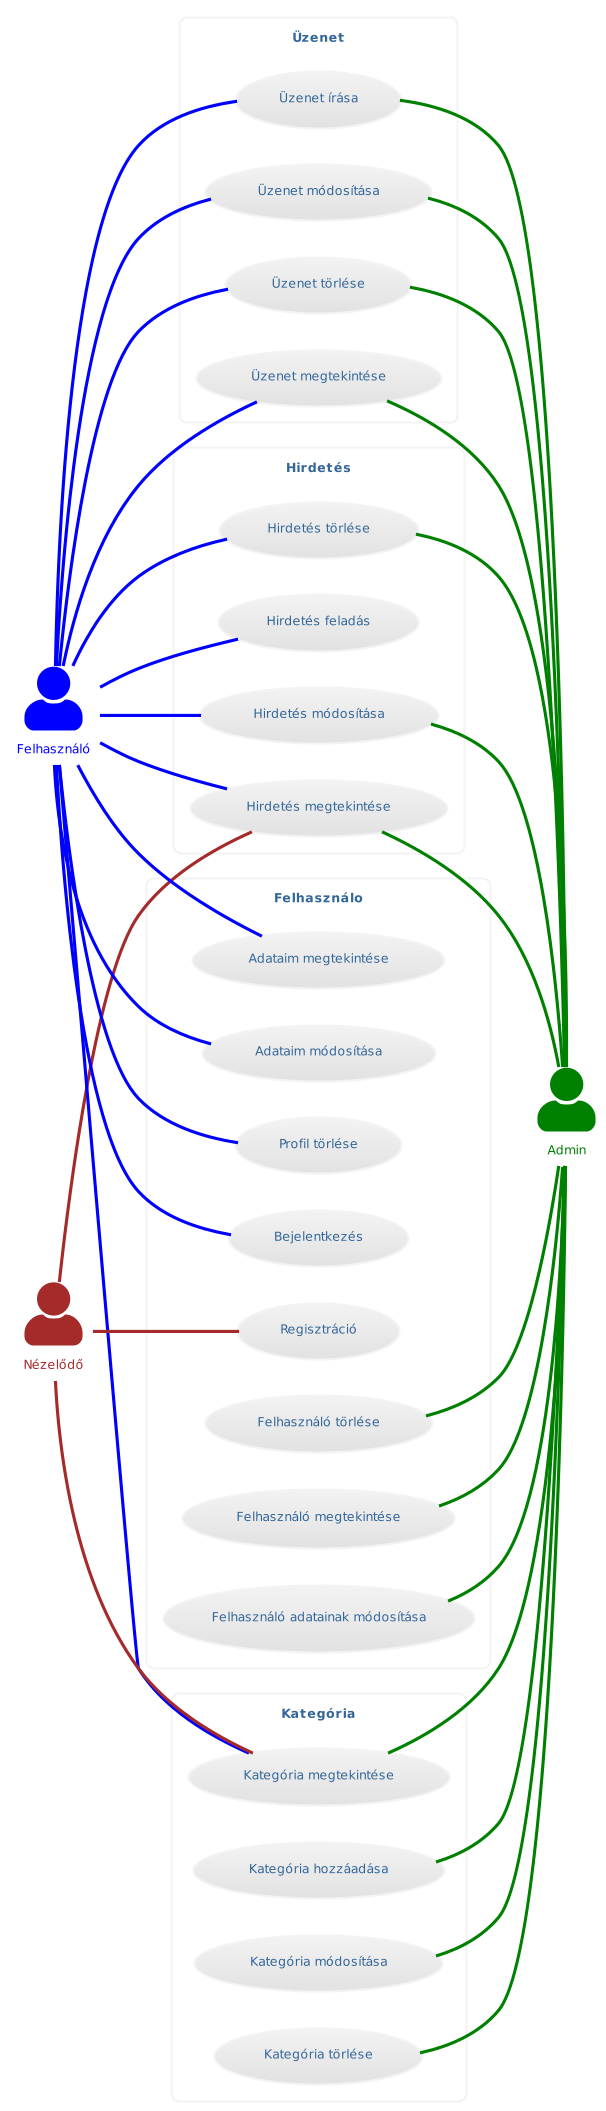
\includegraphics[width=6cm]{./tervezes/useCase}
		\caption{Használati eset (Saját készítés)} 
		\label{useCase}
	\end{figure}
	\Aref{useCase}.~képen látható használati eset ábra magyarázata következik:
	Fontosnak tartom megemlíteni azt, hogy itt ezen az ábrán nem minden funkció kerül megjelenítésére, csak az általam vélt  legfontosabbak. Többet megtudhat \aref{ch-felhasznaloi}.~fejezetben. Az ábrán három darab actor látható.
	\begin{enumerate}
		\item Nézelődő: ennek a szerepnek van a legkevesebb funkciója, ő az aki csak a már meglévő hirdetéseket és kategóriákat tudja megtekinteni, illetve képes még regisztrációra is, ami további meglévő funkciók használata miatt szükséges.
		\item Felhasználó: ő képes a saját adatainak módosítására, a profil törlése is. Neki van már lehetősége saját hirdetéseket létrehozni és ezeket kezelni, valamint már van lehetősége üzenetet küldeni egy másik felhasználónak.
		\item Admin: neki már van lehetősége a kategóriákkal kapcsolatos műveletek elvégésére is. Szintén képes üzenetet küldeni bárkinek, ő képes már felhasználókat és hirdetések törölni az adott esetben.
	\end{enumerate}
	\section{Logó}
		Az adatbázis alapú webalkalmazásomhoz készítettem el egy logót is, ami látható a projektem bejelentkezés és regisztrációs oldalon, illetve magán a navigációs sávon is. A logó elkészítéséhez segítségül vettem az interneten található képeket, majd ezeket összeszerkesztettem, végül pedig Microsoft PowerPoint-ban található funkció segítségével adtam a logónak egy művészi effektust. \Aref{logo}.~ábrán megtekinthető a logó. Az alkalmazásomban szintén egy, az interneten található képet használtam háttérképként. \cite{Logo, Hatterkep}
		\begin{figure}[ht!]
			\centering
			
\includegraphics[width=5cm]{./tervezes/logo}
			\caption{Logó (Saját készítés)} 
			\label{logo}
		\end{figure}
	
	\section{Egyéb}
		Amit még érdekesnek tartotok megemlíteni az olvasóban felmerülhet az a kérdés, hogy a Magyarország területén található vármegyékben elhelyezkedő városokat honnan gyűjtöttem össze. Ezen szükséges információkat a KSH, azaz Központi Statisztikai Hivatal oldalán található Excel táblázat alapján sikerült összegyűjtenem. Azonban sajnálatos módon ez 2015-ös információk alapján lett elkészítve, azóta nagy valószínűséggel néhány adat már elavult benne. \cite{KSH}

	\chapter{Fejlesztés}		
	\section{A fejlesztéshez alkalmazott eszközök és technológiák}
		A következő alszakaszokban a fejlesztéshez használt eszközökről és technológiákról lesz majd szó. Részletezni fogom azokat az eszközöket és technológiákat, melyeket a fejlesztés során használtam és alkalmaztam.
	\subsection{Laravel}\label{sc-laravel}
		A Laravel egy nyílt forráskódú, PHP webkeretrendszer, ami MVC tervezési mintán alapszik. Az MVC a Model-View-Controller rövidítése. Ez az egyik legősibb tervezési minta.
		\begin{enumerate}
			\item Model (magyarul: modell): ez az adatokat kezelő réteg, az adatok tárolásáért és visszaolvasásáért felelős.
			\item View (magyarul: nézet): ez a réteg felhasználói felületek megjelenítéséért illetékes. 
			\item Controller (magyarul: vezérlő, kontroller): a felhasználói műveletek megfelelő kezeléséért ez a réteg a felelős.
		\end{enumerate}
		Az elképzelése röviden az, hogy van egy modell és ha ez módosul, akkor erről értesíteni kell az összes nézetet. Minden nézet pontosan ugyanazon a vezérlőn tudja módosítani a modellt. Mivel három részre van bontva, ezért van ennek a tervezési mintának néhány előnye is. Ilyen például ha lecseréljük az egyik réteget, akkor a többihez nem kell már hozzányúlni, amivel pénzt és időt is lehet spórolni. Előnye még az is, hogy egy modellnek lehet több nézete is. Pozitívumok közzé sorolható az még, hogy számos alapvetőnek tekinthető funkcióhoz lehetséges használni néhány szükséges parancs megadásával. Például a webes alkalmazásomban használtam a laravel breeze-hez\footnote{Ez tulajdonképpen egy alap funkciókat tartalmazó csomag.} tartozó funkciókat. Ezzel különféle autentikációhoz kapcsolódó funkciókat lehet használni, ebbe beletartozik például a bejelentkezés, a regisztráció és a felhasználóval kapcsolatos adatok módosítása is. Még használtam egy olyan parancs által megadható funkciót is, ami a lapozás megvalósítását teszi lehetővé. Ezeknek a pozitívumoknak köszönhetően szerintem a aravel az nagyon megkönnyítheti a fejlesztők számára a munkavégzést. 
		\cite{Kusper, Laravel}
	\subsection{PHP}
		A PHP egy szerveroldali szkriptnyelv, amelynek a segítségével dinamikus weboldalakat lehet vele létrehozni. Azt érdemes még róla tudni, hogy nyílt forráskódú. Ezen kívül még a következő feladatok megvalósítására lehet használni:
		\begin{enumerate}
			\item Parancssoros szkripttelés: itt lehetőségünk van arra, hogy úgy futtassunk egy PHP szkriptet, hogy nem használunk se böngészőt, se semmilyen szervert sem.
			\item Asztali alkalmazások készítése: grafikus felhasználó felülettel ellátott asztali alkalmazások esetén a PHP nem a legjobb választás, azonban van lehetőségünk arra, hogy platformfüggetlen alkalmazások megvalósítsunk.
		\end{enumerate}
		\cite{PHP}
	\subsection{MySQL}
		A MySQL nem más, mint egy nyílt forráskódú adatbázis kezelő rendszer. A MySQL egy relációs adatbázis, ahol az adatokat különböző táblákban vannak eltárolva. Az eltérő táblákban szereplő mezők között lehetnek különféle kapcsolatok is. Ilyen lehet például az egy-az-egyhez kapcsolat vagy egy-a-többhöz reláció. A MySQL adatbázisok szerverére jellemző, hogy gyorsak, megbízhatóak és skálázhatóak.
		\cite{MySQL}
	\subsection{PhpMyAdmin}
		A phpMyAdmin egy ingyenes szoftver, ami arra szolgál, hogy kezelje a MySQL-nek az adminisztrációját weben keresztül. A phpMyAdmin segítségével elvégezhetők a legtöbb adminisztratív feladatok, ideértve az adatbázis létrehozását, lekérdezések futtatását és felhasználói fiókok hozzáadását. \cite{PhpMyAdmin}
	\subsection{XAMPP}
		Az XAMPP nem más, mint egy PHP fejlesztői környezet. Az XAMPP egy angol mozaikszó, melyben az X platformfüggetlenséget jelenti, A az Apache-t jelöli, M a MySql-t fejezi ki, az egyik P a PHP utal, míg a másik P pedig a Perlt jelöli. Az Apache az nem más, mint egy webszerver. Az XAMPP rendszerben található Apache webszerver, ami csak helyi fejlesztést tesz lehetővé számunkra. A Perl pedig egy programozási nyelv. Az XAMPP-ról még azt érdemes tudni, hogy ingyenesen használható és rendkívül egyszerű telepítése, illetve a használata. \cite{XAMPP}
	\subsection{Visual Studio Code}
		Ez egy IDE (integrált fejlesztői környezet), ami ingyenes használható és az egyik legelterjedtebb és legnépszerűbb a fejlesztők körében. Fontosnak tartom megemlíteni, hogy a Visual Studio Code-ban van lehetőség különféle kiegészítők (angolul: extension) letöltésére is, például van lehetőség a python programozási nyelv vagy egy programozási nyelvhez tartozó szintaxis kiemelő letöltésére, illetve ezek használatára. Ezeken kívül pedig tartalmaz még beépített parancssort is, ami nagyon kényelmesé teszi ennek az IDE-nek a használatát. 
	\subsection{GitHub}
		A GitHub-ról azt érdemes tudni, hogy ez egy verziókövető rendszer. Ezek a rendszerek képesek állományok tartalmi változásait követni, azt is képesek megmondani, hogy ki és mikor módosította azokat, valamint van lehetőség arra is, hogy korábbi állapotokat is képes előállítani. A main branch-be feleltethető meg a fő ágnak, amiből van lehetőség elágazások (angolul: branch) is létrehozni. Az elágazásokat arra valóak, hogy a fejlesztési funkciókat elkülönítsük és arra is, hogy úgynevezett pull requestek-nél a nálunk magasabb pozícióban lévő munkatárs leellenőrizze az elkészült munkánkat és, ha helyesnek gondolja csak akkor kerül be a main branch-be. Még arra is használhatjuk, hogy kísérletezzünk vagy akár hibajavítások elvégzésére is lehet használni.
	\subsection{GitHub Desktop}
		A GitHub Desktop egy ingyenesen használható alkalmazás, aminek a segítségével tudunk dolgozni a GitHub-on vagy Git tárhely szolgáltatásokon tárolt fájlokkal. Én ezt az eszközt azért szeretem használni, mivel megkönnyíti és felgyorsítja számomra a munkavégzés, illetve azért is, mert ennek a használatához nem kell a terminálban beírni a Git-hez tartozó parancsokat, hanem egy-két kattintás segítségével könnyedén elvégezhetek egy konkrét parancsot. \cite{GitHubDesktop}
	\subsection{HTML}
		A HTML egy angol eredetű mozaikszó, aminek a jelentése HyperText Markup Language (magyarul: hiperszöveges jelölőnyelv). Ezt a nyelvet weboldalak készítéséhez szokás használni. Az én projektemben ezt a nyelvet a blade-ek készítésénél használtam. A bladek-ről többet megtudhat \aref{sc-blade}.~alfejezetben.   
	\subsection{Tailwind CSS}\label{sc-tailwind}
		Tailwind CSS használatával a felhasználói felületeket lehet kialakítani, ez csak külsőleges formázást jelent, tehát csak és kizárólag esztétikai szépítésre szolgál. Érdemes még róla tudni, hogy gyors, megbízható, rugalmas és nincsen futási ideje, azaz azonnal megtörténik a változás, nem kell rá várni semmit sem. A fejlesztés során néhány a webalkalmazásomban található gomb kinézetét és figyelmeztetések esetén megjelelő stílust használtam fel, ezeknek a forrása megtekinthetőek az irodalomjegyzékben \cite{tailwind, FlowBite}
	\subsection{JavaScript}\label{javascript}
		A JavaScript az egyik szkript- vagy programozási nyelv, aminek a segítségével van lehetőség bonyolultabb funkciók megjelenítésére a weboldalakon. Lehetővé teszi például egy dinamikusan frissülő tartalom létrehozását vagy akár képek animálását is. Ezeken kívül még nagyon sok mindenre használható még. A projektemben használtam a JavaScript-et ahhoz, hogy amikor vármegyét választok ki egy legördülő listából, akkor egy másik listában csak az előzőleg kiválasztott vármegyébe tartozó város jelenjenek meg. A másik ahol szintén használtam az pedig a szűréshez tartozó részeket jelenítem meg vagy nem, annak a tükrében, hogy be van pipálva egy checkbox (magyarul: jelölőnégyzet) vagy nem.
		
	\chapter{Tesztelés}
		A tesztelésre azért van szükség, hogy az alkalmazásomban megtaláljam az esetleges hibákat, amiket kijavítva növelhetem a szoftverem minőségét és megbízhatóságát. Abban sajnos nem lehetek biztos, hogy a tesztelés elvégzése után nem lesznek már hibák. A tesztelés során kettőféle tesztelési technikát alkalmaztam. Ezek pedig a következők:
		\begin{enumerate}
			\item Fehérdobozos (angolul: white-box): a forráskód alapján íródnak a tesztesetek.
			\item Szürkedobozos (angolul: grey-box): amikor a forráskódnak csak egy rész ismert és csak ez alapján íródnak a tesztesetek.
		\end{enumerate}
		Azonban van egy harmadik fajta is, amit nem alkalmaztam. Az nem más, mint a feketedobozos (angolul: black-box), amikor a tesztesetek a specifikáció alapján íródnak.
		\cite[26-29.~oldal]{Kusper}
	\section{A teszteléshez alkalmazott eszközök és technológiák}
			A következő alszakaszokban a teszteléshez használt eszközökről és technológiákról lesz majd szó. Kitérek majd arra is, hogy pontosan mit is jelentenek, miket lehet velük tesztelni és az előnyük és hátrányaikról is ejtek majd pár gondolatot.
	\subsection{Manuális teszt}
		Manuális teszt az azt jelenti, hogy a tesztelő végig próbálgatja saját magától a funkciókat és leellenőrzi azok működését, illetve helyességét. Az ilyenféle tesztelés végzésekor nem alkalmazunk semmilyen automatizált tesztet. Én fejlesztés közben folyamatosan végeztem manuális tesztelést, abból kifolyólag, hogy megbizonyosodjak az elkészült funkció helyességéről, illetve, hogy feltárjam vele az esetleges hibákat, amiket nem vettem észre vagy még nem gondoltam rá. Az én meglátásom szerint a manuális tesztelésnek a legnagyobb hibája az, hogy minden lehetséges kombinációt ki kell próbálnunk ahhoz, hogy bebizonyosodjunk arról, hogy a készített funkció a megfelelő módon működik. Még szintén hátrány lehet az, hogy rendkívül költséges lehet a manuális tesztelés. Végül pedig az, hogy az emberek nagyobb százalékban hibáznak, ami érthető is, hiszen tévedni emberi dolog. Azonban vannak előnyei is, ezek pedig véleményem szerint a következők lennének. Az első ilyen az lenne, hogy, ha van valamilyen hiba, akkor azt nagy valószínűséggel hamarabb észre lehet venni, amivel pénzt és időt is lehet spórolni. A másik ilyen előny az pedig, hogy a tesztelőnek van megfelelő intelligenciája ahhoz, hogy kiszűrje az esetleges hibákat, ellenben az automatizált tesztekkel szemben. 
		
	\subsection{Cypress}
		A Cypress egy NodeJS-ben\footnote{Ez egy ingyenes, nyílt forráskódú futtatókörnyezet, amellyel webes alkalmazásokat, szervereket is lehetséges létrehozni.} írt frontend tesztelési keretrendszer. Ahhoz, hogy tudjuk futtatni a Cypress-t, ahhoz előtte telepíteni kell a NodeJS-t. A Cypress segítségével tudunk készíteni végponttól végpontig tartó-, komponens-, integrációs- valamint a unitteszteket is.
		Az imént felsorolt teszt típusok jelentése a következő:
		\begin{enumerate}
			\item Végponttól végpontig tartó teszt: ennél a típusnál a szoftver funkcionalitását és teljesítményét teszteljük a kezdetektől a végéig, ami a vég felhasználok által megvalósított interakciókat szimulálja valós adatokkal.
			\item Komponensteszt: ez nem más, mint, amikor a rendszernek csak egy önálló komponensét teszteljük.
			\item Integrációs teszt: ez egy olyanféle teszt, aminél legalább kettő különböző komponens együttműködését teszteljük.
			\item Unitteszt (magyarul: egységteszt): ez egy olyan teszt, ami a metódusokat teszteli le. Itt nézzük meg, hogy a tényleges visszatérési érték azonos-e az elvárttal. Ez a komponensteszt egyik fajtája.
		\end{enumerate}
		Ezzel a tesztelési keretrendszer segítségével bármit lehet tesztelni ami a böngészőben fut. Nézzük meg néhány előnyét és hátrányát is ennek használatára. Kezdjük a negatívumokkal először. A teszteknek JavaScript nyelven kell íródniuk. Erről többet megtudhat itt \aref{javascript}. Hátrány még az is, hogy egyszerre csak egy ablakban vagy csak egy böngészőben lehetséges a tesztek végrehajtása. Most nézzük meg a pozitívumait is. Az egyik legnyilvánvalóbb ha ránézzünk egy ilyen kódra az, hogy nagyon olvasható bárki számára. Előny még az is, hogy igazi böngészőt használ a tesztek végrehajtására. Ez azért hasznos, mivel a valódi végfelhasználók is igazi böngészőkben fogják használni az alkalmazást, ezért jól lehet velük szimulálni a működését. Még előnynek tekinthető az is, hogy a hálózatól érkező kéréseket lehetséges ellenőrizni a Cypress segítségével.
		\cite{Cypress, Kusper Szoftvertesztles, Katalon, Medium, NodeJS}
		
		A szemléltetés kedvéért szeretné, Önnek bemutatni, hogy hogyan is kell elképzelni egy ilyenféle tesztet. \Aref{cypress-teszt}.~kódon megtekinthető.
		
		\lstinputlisting[caption={Egy Cypress teszt egy hirdetés hozzáadására}, label=cypress-teszt, style=user1, language=JavaScript]{./teszteles/add.js}
		
		Itt a visit (magyarul: meglátogat) metódus segítségével lehetséges egy konkrét útvonalra eljutni. Ezután bejelentkezni szükség, mivel csak akkor van lehetőség hirdetés hozzáadására. Id, azaz valamilyen azonosító alapján szükséges megkeresni a form-on az adatok megadásának a helyét. Ahol mi adunk meg valamilyen információt, ott a type (magyarul: begépel) metódus segítségével tehetjük meg. Ahol legördülő menüből kell kiválasztani a szükséges adatokat, ott pedig a select (magyarul: kiválaszt) metódussal lehetséges. Ezen kívül még két darab kép hozzáadása is látható még, ezt az attachFile (magyarul: fájl csatolása) metódussal történik, azonban ehhez szükséges még egy csomagot letölteni, de ezt csak megemlítettem, mivel többet erről nem lesz szó. Gombokat lehetséges szöveg alapján megkeresni és utána rákattintani, ez pedig a contains (magyarul: tartalmaz) és click (magyarul: rákattint) metódusokkal történhet meg. Végezetül pedig egy átirányítása megvalósítása látszik, ha minden sikerrel zárult. Tehát véleményem szerint kijelenthető, hogy Cypress tesztek írása egyszerű és nagyon érthető még akár egy hétköznapi ember számára is.
		
	\subsection{Tesztek eredménye}
		Az elvégzett Cypress tesztek eredményessége alapján megállapítható, hogy jelentős mértékben sikeresek voltak. Néhányszor előfordult, hogy bizonyos esetek eleinte nem feleltek meg a teszteseteknek, de végül sikeresnek bizonyultak. Összességében a véleményem szerint a tesztek nagy sikerrel javították az apróhirdetés webalkalmazásomat.   
		
	\chapter{Felhasználói dokumentáció}\label{ch-felhasznaloi}
		Ebben a fejezetben szó lesz majd, arról, hogy különböző jogosultságú felhasználóknak milyen lehetőségei vannak a webes alkalmazásom használata során. Minden ebben a fejezetben lévő alfejezetben szereplő jogosultsághoz szinte csak azokat a funkciókat említem majd meg, amiket csak ők tudnák használni. A különböző szerepű felhasználókról \az{\ref{sc-plantuml}} alfejezetben már megemlítettem róluk pár szót. Az alkalmazásomban található ikonokat egy interneten lévő oldalon találtam meg, az irodalomjegyzékben megtalálható a keresett oldal.\cite{Ikon} 
	\section{Admin}
		Az admin (magyarul: adminisztrátor) van néhány szükséges egyedi funkció az alkalmazásomnak. Az adminisztrátoroknak nagyon fontos szerepük bármilyen alkalmazás életében. Az webes projektemben a következő admin funkciókat készítettem el.
	\subsection{Felhasználókkal kapcsolatos művelet}
		Az én meglévő tudásom birtokában úgy gondoltam, hogy a csak és kizárólag törölni tudjon már regisztrált felhasználókat. Admin jogosultságú felhasználókat nem lehetséges kitörölni, azaz amennyiben van több ilyen, akkor nem tudják kitörölni egymást. A törlendő felhasználók megtalálása miatt egy keresés funkciót is implementáltam bele, aminek a segítségével könnyeben megtalálható a keresett felhasználó.
	\subsection{Kategóriákkal kapcsolatos műveletek}\label{sc-kategoria}
		Ennek a jogosultságnak a birtokában képes új kategóriát hozzáadni, módosítani már meglévőt és még képes törölni is, amennyiben szükséges. \Aref{kategoria-muveletek}.~ábrán a kék színű ikon segítségével módosítani lehet a kategóriát, a piros színűvel pedig törölni. A képen nem látszik viszont van ott egy gomb, aminek a segítségével tudunk új kategóriát hozzáadni.
		\begin{figure}[ht!]
			\centering
			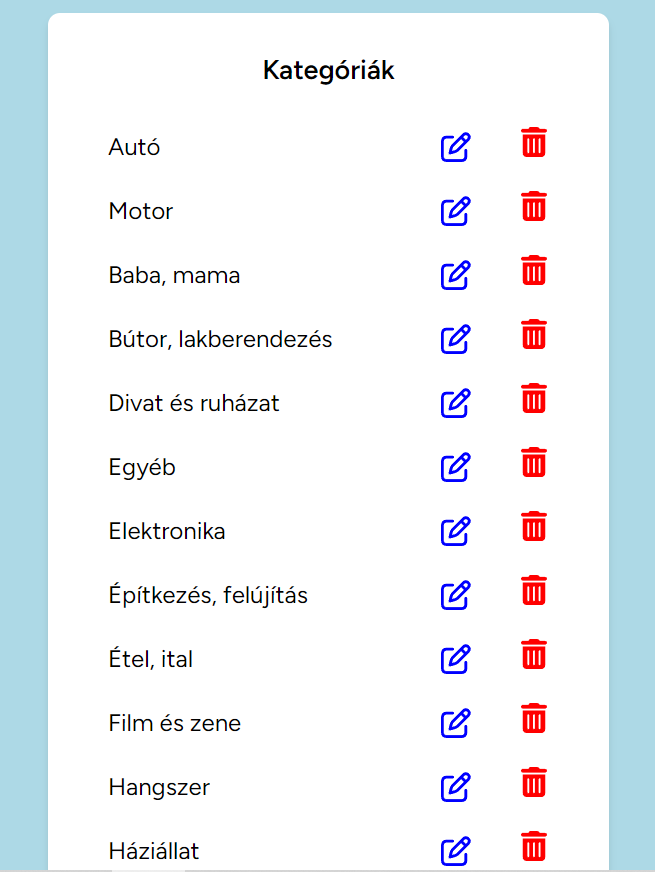
\includegraphics[height=8cm]{./felhasznaloi/kategoria}
			\caption{Kategóriák (Saját készítés)} 
			\label{kategoria-muveletek}
		\end{figure} 
	\subsection{Vármegyével és városokkal kapcsolatos műveletek}
		Itt az admin jogosultságú felhasználó képes új vármegyét hozzáadni, meglévőt módosítani, illetve törölni. Szintén képes még különböző vármegyékhez hozzáadni új városokat, meglévőt módosítani és törölni. \Aref{varmegye-varos-muvelet}.~ábrán a zöld színű ikon segítségével lehet megtekinteni az adott vármegyéhez tartozó városokat megjeleníteni, ez ugyan úgy épül fel, mint az imént említett kategóriák \aref{sc-kategoria}.~alfejezetben. A kék színű ikon segítségével módosítani lehet a kategóriát, a piros színűvel pedig törölni. A képen nem látszik viszont van ott egy gomb, aminek a segítségével tudunk új vármegyét hozzáadni.
		\begin{figure}[ht!]
			\centering
			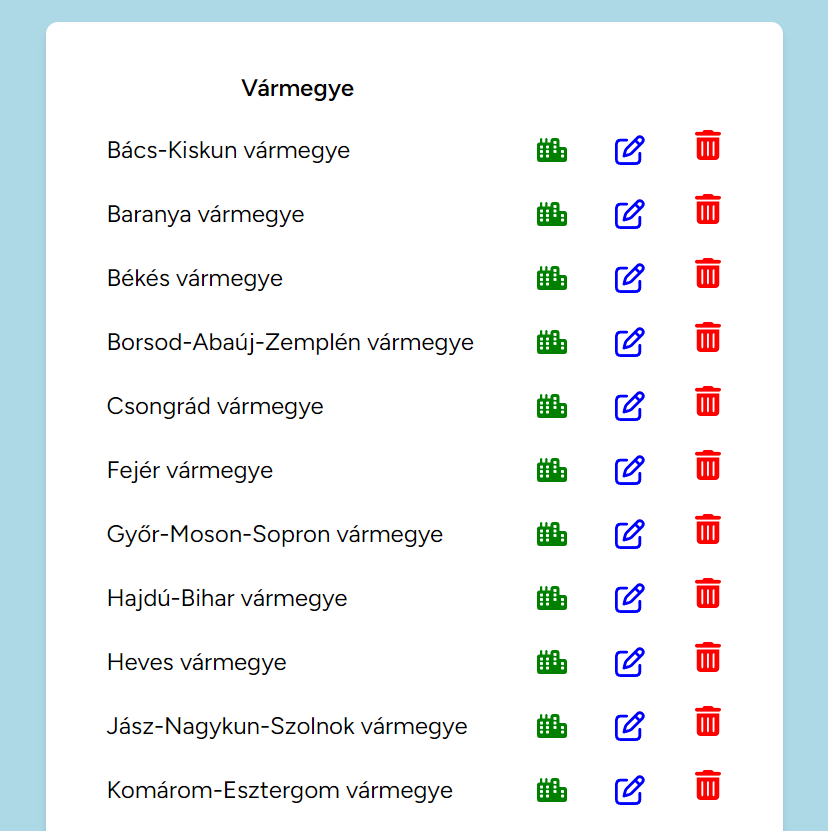
\includegraphics[height=9cm]{./felhasznaloi/varmegye}
			\caption{Vármegyék (Saját készítés)} 
			\label{varmegye-varos-muvelet}
		\end{figure}
	\subsection{Hirdetéssel kapcsolatos műveletek}
		Ez lenne az egyetlen kivétel, itt a sima felhasználó is képes módosítani vagy törölni a saját hirdetéseit. Képes a már az összes meglévő hirdetéseket módosítani, illetve törölni azokat, ha valamilyen oknál fogva nem megfelelő nyelvezetet vagy képet használ, új képet nem tud hozzáadni az admin, csak és kizárólag törölni képes. Az adminisztrátor jogosultsággal rendelkező felhasználók nem képesek a vármegye, város megváltoztatására, hiszen ezt a hirdetés tulajdonosának a feladata, amennyiben szükség lenne rá.
	\section{Felhasználó}
		A következő alfejezetekben csak a sima felhasználó egyedi funkcióijáról lesz szó.
	\subsection{Hirdetéssel kapcsolatos műveletek}
		Regisztrált felhasználóként van arra lehetőség, hogy a hirdetéseivel kapcsolatos műveleteket végezzen el a felhasználó, legyen szó akár csak azok megtekintéséről, módosításairól vagy törléseiről. Ő már képes új hirdetések létrehozni, ami \aref{hirdetes-hozzadas-muvelet}.~ábrán lesz látható.
		\begin{figure}[ht!]
			\centering
			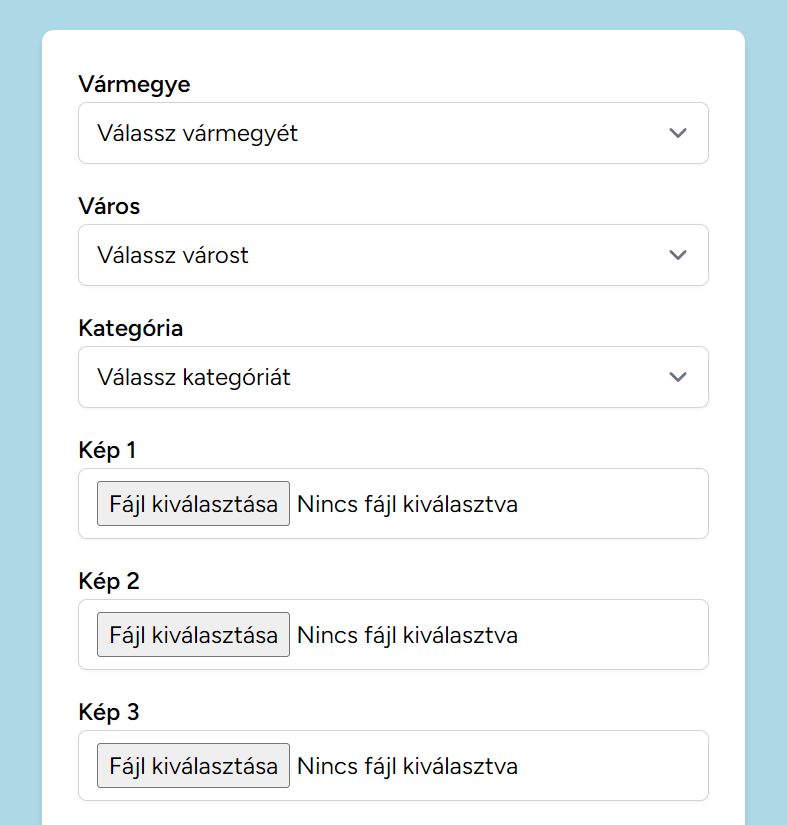
\includegraphics[height=7cm]{./felhasznaloi/hozzadas1}
			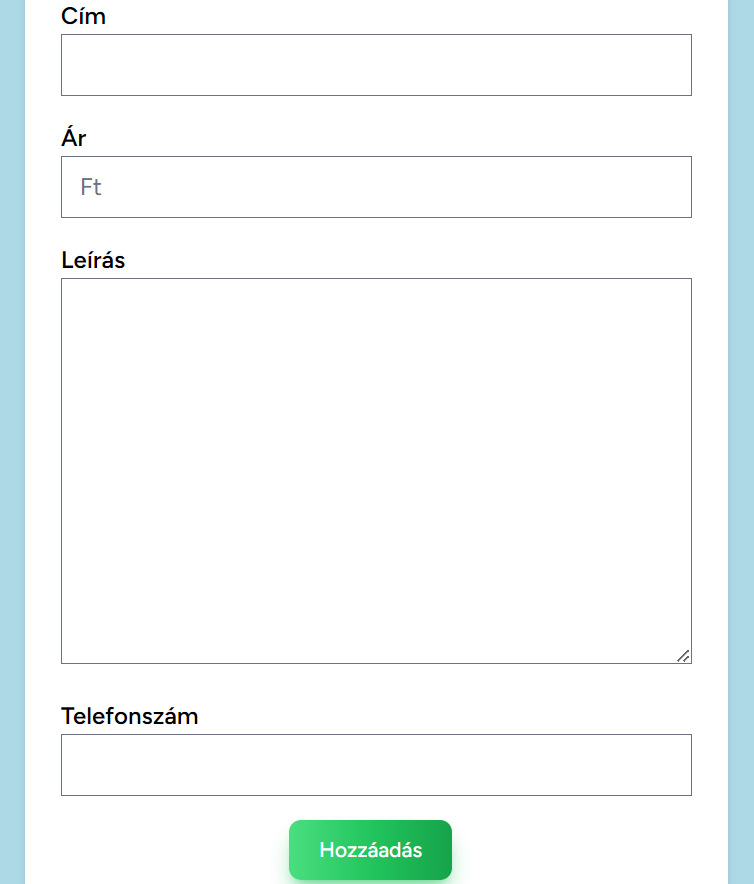
\includegraphics[height=7cm]{./felhasznaloi/hozzadas2}
			\caption{Új hirdetés hozzáadása (Saját készítés)} 
			\label{hirdetes-hozzadas-muvelet}
		\end{figure}
		\Aref{hirdetes-hozzadas-muvelet}.~ábrán magyarázata következik. A vármegyét egy legördülő listából lehet kiválasztani, ha ezt megtettük csak utána tudjuk majd a várost kiválasztani szintén legördülő listából. A hirdetés kategóriáját is ilyenféle módon választhatjuk ki. A címét, árát és leírását pedig a felhasználó adja majd meg. Ezek voltak a kötelezően megadandó információk. Telefonszámot, illetve képeket nem szükséges megadni. A megadható képek számát limitáltam 5 darabra.
	\section{Nézelődő}
		Ő nem rendelkezik semmilyen jogosultsággal sem, ezért is nincsen egyedi funkciója ennek a szerepkörnek. Ő csak a kategóriákat képes megtekinteni, illetve a meglévő hirdetéseket tudja megnézni. Keresésre és szűrésre is van itt lehetősége. Ezekről \aref{egyeb-funkciok}.~alfejezetben olvashat többet.
	\section{Egyéb funkciók}\label{egyeb-funkciok}
		\begin{enumerate}
			\item Keresés: a hirdetéseknél van arra lehetőség, hogy keresni lehessen, ez a hirdetés címe alapján lehetséges.
			\item Szűrés: van arra lehetőség, hogy szűrjünk ára, vármegyére, városra vagy kategóriára is.
			\item Rendezés: a hirdetéseket rendezhetjük ár szerint növekvő, csökkenőbe vagy lehet alapértelmezett is.
				\begin{figure}[ht!]
				\centering
				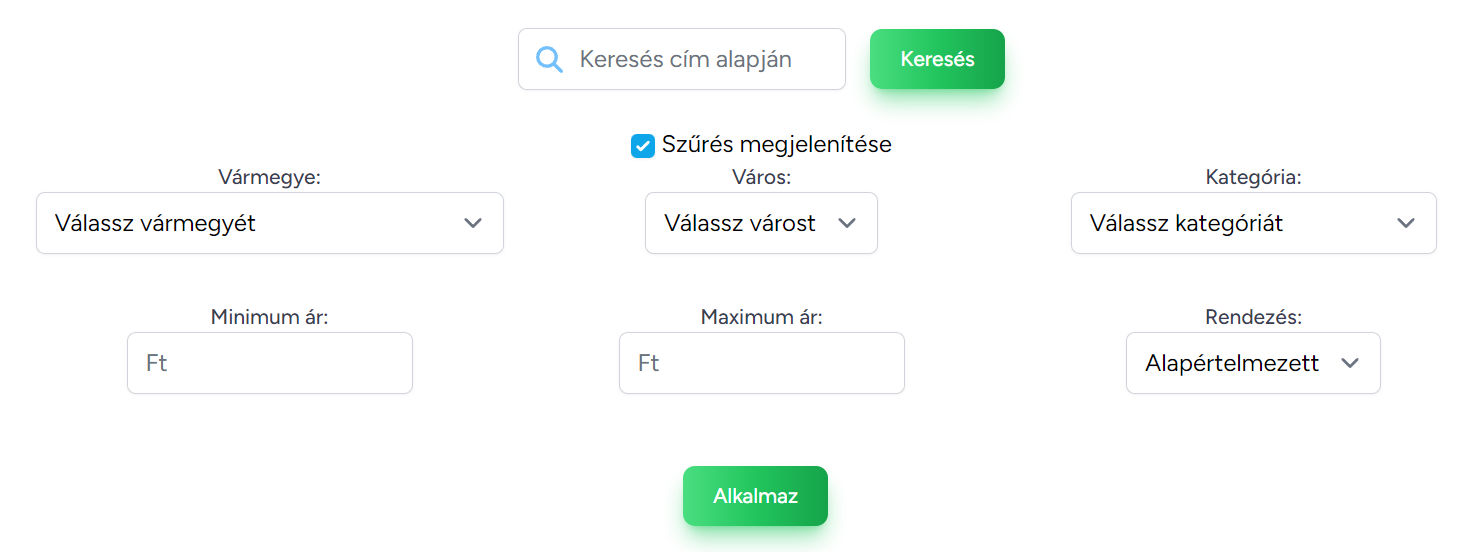
\includegraphics[width=13cm]{./felhasznaloi/kereses-szures}
				\caption{Keresés, szűrés és rendezés (Saját készítés)} 
				\label{kereses-szures-muvelet}
			\end{figure}
			\item Üzenetek: a regisztrált felhasználók vagy adminisztrátorok képesek üzenetek küldeni egymásnak, ezeket megtekinteni, módosítani vagy törölni a saját maguk által korábban elküldött üzeneteket is. Itt a megkülönböztetés és a felismerés céljából az a felhasználó, aki adminisztrátor jogosultsággal rendelkezi, akkor annak zöld színnel jelenik meg a neve. Ezáltal a sima felhasználók tudhatják, hogy valóban egy ilyen jogosultságú felhasználótól kaptak szöveges üzentet.
			\item Profil módosítása: a webes alkalmazásomban adva van a lehetőség arra, hogy a regisztrált felhasználó tudják módosítani a saját adataikat, illetve képesek törölni a profiljukat is. Az adminisztrátor nem képes arra, hogy módosítsa a felhasználók adatait, csak törölni tudja őket.
			\item Saját hirdetések listázása: a felhasználó által létrehozott hirdetéseket megtekintésére, módosítására és törlésére ezen a helyen van lehetőség rá. Itt szinten van ara mód, hogy keresni tudjunk a saját hirdetéseink között, ez a hirdetés neve alapján történhet meg.
			\item Hirdetések listázása kategóriák alapján: ez lenne azaz oldal, amit a felhasználók elsőnek látnának meg, tulajdonképpen ez a főoldal. Ez hasonló, mint a szűrés funkció, azonban itt a kategória nevére rákattintva már rögtön megjelenik az adott kategóriába tartozó hirdetéseket.
		\end{enumerate}
	
	\chapter{Fejlesztői dokumentáció}
		A fejezetben szó lesz az alkalmazásom felépítéséről, ezen kívül még szót ejtek majd a jogosultságkezelésről is, hogy hogyan oldottam meg és milyen lehetőségeim voltak a fejlesztés során.
	\section{Az alkalmazás felépítése}
		Ebben az alfejezetben beszeretném mutatni Önöknek az alkalmazásom fő komponenseit kódrészletek segítségével a könnyebb megértés reményében. Egy nagyon keveset már megemlítettem korábban \aref{sc-laravel}.~alfejezetben, de nem mindent, most lépésről lépesre elmesélem, hogy hogyan lehetséges megjeleníteni egy konkrét információkat az adatbázisomból.
	\subsection{Adatbázis kapcsolat létrehozása}
		Magát az adatbázist többféle módon van lehetőségünk létrehozni, de ezekbe most nem mennék bele. Most itt még azt kell megemlítenem, hogy a projektemben ezt hogyan állítottam be. Ehhez meg kell keresni a projektben a .env nevű fájlt és meg kell adni néhány információt. A következőket szükséges megadni.
		\begin{enumerate}
			\item DB\_CONNECTION (magyarul: adatbázis kapcsolat): itt magát az adatbázis fajtáját kell megadnunk. Alapértelmezetten MySql van megadva. 
			\item DB\_HOST (magyarul: adatbázis kiszolgáló): ez az adatbázis IP-címe lenne.
			\item DB\_PORT (magyarul: adatbázis port): ennek a segítségével tudunk kapcsolódni az adatbázis szerverhez. 
			\item DB\_DATABASE (magyarul: adatbázis neve): itt az magát az elnevezését kell megadnunk.
			\item DB\_USERNAME (magyarul: felhasználónév az adatbázishoz): meg kell adnunk egy felhasználónevet, amelyet az alkalmazás használ a belépéshez.
			\item DB\_PASSWORD (magyarul: jelszó az adatbázishoz): a belépéshez meg kell adnunk még egy jelszót is.
		\end{enumerate}
	\subsection{Migráció}
		A migrációk segítségével tulajdonképpen az adatbázis struktúráját tudjuk definiálni. Van arra lehetőség, hogy egy migrációs fájlt egy parancs segítségével lelehessen generálni struktúra szintjén, de már a benne szükséges mezőket és az esetleges különböző megszorításokat már nekünk kell definiálni. A következő parancs segítségével lehetséges egy migrációs fájlt generálni:
		\begin{center} 
			php artisan make:migration create\_név\_table .
		\end{center}
		Következőnek nézzük azt meg, hogy hogyan is épül fel egy migrációs fájlt, konkrétan az a hirdetéshez tartozó.
	
		\lstinputlisting[caption={Egy migrációra példa kód}, label=kod-migracio, style=user1, language=PHPOwn]{./fejlesztoi/hirdetes.php}
		
		Látható tehát, hogy egy mezőt úgy szükséges megadni, hogy \$table-->mező típusa, majd zárójelbe a mező nevét.
		A 15.~sorban az elsődleges kulcs megadása látható. Az alatta lévő sorban pedig egy olyan mezőt hoztam létre, ami majd egy másik migrációs fájlból kapja majd meg az értékét, tehát ez egy idegen kulcs. A 25.~sorban pedig az imént említett mezőre így lehetséges hivatkozni. Itt ennek a sornak végén lévő kód az azt jelenti, hogy ha kitörlődik az adott felhasználó, akkor a hirdetés is törlődni fog vele együtt. Alapértelmezetten egyik mező értéke sem lehet nulla, ha azonban szükségünk van rá, akkor meglehet tenni úgy, ahogyan én a 22.~sorban csináltam. Ha elkészültünk a migrációs fájlokkal, akkor a következő parancs segítségével lehet majd végrehajtani azt:
		\begin{center}
			php artisan migrate .
		\end{center}
	\subsection{Modell}
		A laravel már tartalmazza az eloquent-et, ami egy ORM (angoul: Object-Relational Mapping, magyarul: objektum-relációs leképzés). Amikor ezt használjuk, akkor minden egyes adatbázis táblához tartozik egy modell is, aminek a segítségével interaktálni tudunk a táblával. Az ilyenféle modellek használatával lehetséges beszúrni, módosítani vagy törölni az adott adatbázis táblából. Itt a modellekben még megadhatunk különféle metódusokat is és még itt van lehetőség az eloquent kapcsolatok megadására is. Ezekre még majd kitérek a példa bemutatása során.\cite{Laravel}
		
		\lstinputlisting[caption={Egy modellre példa kód részlet}, label=kod-modell, style=user1, language=PHPOwn]{./fejlesztoi/hirdetesModell.php}
		
		\Aref{kod-modell}.~kódrészleten a 6.~és 7.~sorban az adatbázis tábla neve és elsődleges kulcs megadása látható. Rögtön alatta pedig az látszik, hogy egy tömbbe megadom a kötelezően megadandó mezők nevét, amiknek az értékük nem lehet üres. Itt található még egy belongsTo és egy hasMany kapcsolatra egy példa. Az első azt röviden az azt jelenti, egy modell egy másik modellhez tartozik, azaz, hogy egy hirdetés egy felhasználóhoz tartozik. Míg az utóbbi azt azt jelenti, hogy egy modell több modellhez tartozik, azaz egy hirdetéshez több kép is tartozhat. Egy modell létrehozása a következő parancs segítségével történhet meg:
		\begin{center} 
			php artisan make:model név .
		\end{center}
	
	\subsection{Kontroller}\label{sc-kontroller}
		A kontrollerek tulajdonképpen arra használatosak, hogy a különböző kérésékhez szükséges metódusokat itt definiálhatjuk. A kontrollerekben általában sokféle metódusokat írhatunk, azonban alap esetekben a következő lehetnek. Lehet index nevű, ami az összes adat vagy más néven erőforrások megjelenítésére szolgál, lehet még create (magyarul: létrehozás), ami az adatok bekéréséért felelős form, ehhez szorosan kapcsolódik a store (magyarul: tárol, mentés), ami pedig elmenti a kívánt erőforrást. Beszélhetünk még a show (magyarul: megnéz) és a destroy (magyarul: törlés) metódusokról, az előbbi egy konkrét erőforrást jelenít meg, míg utóbbi segítségével az erőforrást lehetséges kitörölni. Végezetül még két metódus van, az első az edit (magyarul: módosítás), ami a create metódushoz hasonlóan egy form-ot jelenít meg, aminek a segítségével lehetséges az adott erőforrás módosítása. A másik pedig az update (magyarul: módosítás), ez pedig konkrétan módosítja az imént említett edit form-on az eszközölt változtatásokat. Példa képen a show metódust mutatom be Önnek. \cite{Laravel}
	
		\lstinputlisting[caption={Egy kontrollerben lévő metódus}, label=kod-kontoller, style=user1, language=PHPOwn]{./fejlesztoi/hirdetesShow.php}
	
			A következőben röviden megmagyarázom \aref{kod-kontoller}.~kódot. Látható, hogy a hirdetéshez tartozó kontrollerben található a metódus, ami paraméterként kér egy id-t, az id segítségével tudom, hogy pontosan melyik hirdetést szeretném megjeleníteni. Ezután megkeressem az adott bekért id alapján a hirdetést, majd leellenőrzöm, hogy egyáltalán létezik-e, ha nem akkor hibát adok vissza, amit majd a blade tudunk majd felhasználni, ahhoz, hogy értesítsem a felhasználót a hibáról. Végül pedig, ha nincsen hiba, akkor megjelenítem egy másik bladen a felhasználó számára. A compact nevű metódusra, azért van szükségem, hogy a blade-n majd megjeleníteni tudjam a kívánt hirdetést. A bladek-ről többet \aref{sc-blade}.~alfejezetben tudhat meg.  Egy kontroller létrehozása a következő parancs segítségével történhet meg:
		\begin{center} 
			php artisan make:controller névController .
		\end{center}
		  
	\subsection{Web.php}
		A web.php nevű fájl, arra szolgál, hogy a kontrollerekben elkészített különböző metódusokhoz route-t (magyarul: útvonal) rendeljük hozzá. Ez azért szükséges, hogy a böngészőkben eltudjuk érni magát a konkrét blade-t, ami a kontrollerben definiált metódust fogja megvalósítani. Itt még annyit érdemes megemlítenem, hogy a middleware (magyarul: köztes szoftver) segítségével van lehetőség szabályozni, azt hogy ki férhessen hozzá az adott útvonalhoz. A következőben pedig egy útvonalat fogok mutatni, hogy eltudják képzelni, hogy hogyan is nézz ki.
	
		\lstinputlisting[caption={Egy web.php lévő útvonal}, label=kod-utvonal, style=user1, language=PHPOwn]{./fejlesztoi/hirdetesUtvonal.php}
	
		Röviden az látható \aref{kod-utvonal}.~kód részleten, hogy a route és két darab kettőspont után van lehetőségünk a kérést típusát megadni, attól függően, hogy melyik metódust hívjuk meg. Jelen esetben most get (magyarul: kap) található ott, ami tulajdonképpen a listázásért felelős. Gyakran használatosan még a post (magyarul: hozzáadás, beszúrás), a put (magyarul: módosítás) és a delete (magyarul: törlés) elnevezések. Ezt követően következik az első paraméter, ami az elérési útvonal, a másik pedig azon az útvonalon található metódust lesz. Még megtalálható a végen ott egy elnevezés metódus, aminek a segítségével könnyeben tudunk majd hivatkozni a kívánt blade-n. Ennek a használata azért előnyös, mivel így nem kell a teljes útvonalat megadni, ha hivatkozni szeretnénk a metódusra és ha esetlegesen változtatni kellene az útvonalon, akkor azt csak egy helyen elég megtenni, itt a web.php-ben. Ha nem neveznénk el és több blade is használná ezt az útvonalat, akkor mindenhol meg kellene változtatni, ami nem lenne túl szerencsés. A bladek-ről többet \aref{sc-blade}.~alfejezetben tudhat meg.
		
		Megközelítőleg az alkalmazásomban ötven darab útvonal található meg, és ezek közül számosban fennlelhető valamilyen id, azaz azonosító. Erre azért van szükség, hogy a különböző erőforrásokat azonosítani lehessen és azért is, hogy ezeknek a segítségével valamilyen műveletet is lehessen rajtuk végezni. Ide tartozhat a lekérdezés, a hozzáadás, a módosítás és a törlés műveletek. Fontosnak tartom még azt kiemelni, hogy a webböngészőben az URL-ben\footnote{Az angol uniform resource locator kifejezés rövidítése. Ez egy egyedi azonosító, amely egy erőforrást (például egy weboldalt) segít megtalálni az interneten.} lévő azonosítókat lehet módosítani és ennek a dolognak a kivédése érdekében megfelelő lépéseket megtettem. Amennyiben, hogyha a felhasználó például a saját hirdetését kívánja módosítani, akkor az URL-ben láthatja a hirdetés azonosítóját és, ha ezt megváltoztassa, akkor már egy másik hirdetéshez tartozó módosítása nézetet tekintené meg, ami nagy valószínűséggel egy másik felhasználóhoz tartozik, de ez nem történhet meg mivel raktam a programomba az ilyenféle hibák miatt hibakezelést. Ezt átirányítás és megfelelő hiba üzenet segítségével tudatom a felhasználóval. Ha a felhasználó egy nem létező URL-t adna meg, akkor pedig szintén ugyanazokat lépéseket teszem meg, mint az előző, az azonosítóval kapcsolatos problémánál. Amennyiben az adott felhasználó olyan útvonalat ad meg amihez nincsen meg a kellő jogosultsága, akkor vagy szintén átirányítás és hiba üzenet segítségével tudatom vele, vagy pedig, akkor átirányítom a bejelentkezés felületre, mivel ekkor ő még csak egy sima nézelődőnek tekinthető. A bejelentkezés elvégzése után, kellő jogosultság birtokában már képes a kívánt művelet elvégzésére, amennyiben nem adminisztrátor tartozó műveleteket szeretne elérni, kivéve, ha az adott felhasználó már rendelkezik az imént említett jogosultsági szinttel.
	
	\subsection{Blade}\label{sc-blade}
		A blade-k segítségével azokat nézeteket tudjuk definiálni, amiket látni lehet a böngészőben. Tulajdonképpen ez lenne a UI (user interface), azaz a felhasználói felület. Egy hirdetés megjelenítéséért felelős felület szeretném bemutatni, amiről már szó esett az előző két alfejezetben. Ezen \aref{kod-blade}.~kód részleten láthatja meg, ami \aref{ch-fugg}.~fejezetben található meg.
	
		Erről csak röviden szeretnénk beszélni, rögtön az elején van ként részlet, ami említésre méltó. Az extends (magyarul: kibővít) kulcsszó segítségével kitudjuk bővíteni egy másik felületet, a másik kulcsszó pedig a section (magyarul: szekció), ami pedig a kibővített felületen belüli content (magyarul: tartalom) helyére kerül be a taglalt felület. Táblázatos formában jelenítettem meg a hirdetést, és ennek a Tailwind CSS (\ref{sc-tailwind}) segítségével való formázás található még ott. \Aref{sc-kontroller}.~alfejezetben esik szó a compact nevű metódusról, aminek a használata azért volt szükséges, hogy elérjük a \$advertisement (magyarul: hirdetés) változót. Még egy dolgot szeretnénk kiemelni, ami pedig a 36.~sorban olvasható. Erről már volt szó ebben \aref{kod-modell}.~alfejezetben. Itt a modellek miatt tudom ezt megtenni, hogy így megtudjam jeleníteni a hozzá tartozó kategória nevét, ennek a hiányában a hirdetéshez tartozó kategória id-t tudnám csak megjeleníteni.
	\section{Jogosultságkezelés}
		A jogosultságkezelés minden projektnél egy nagyon kulcsfontosságú, lényeges szerepet tölt be, mivel általában szükség van arra, hogy lehessen szabályozni a különböző funkciók használatát. A laravel keretrendszer számos lehetőséget ad számunkra ezen a téren. Ilyen opció például a middleware (magyarul: köztes réteg) vagy a policy (magyarul: szabályzat). Én az utóbbi mellett tettem le a voksomat. Ennek a használata nagyon egyszerű és érthető volt számomra. A policy-ben egy adott modellhez vagy erőforráshoz tartozó autentikációs logikát szükséges implementálni. Egy ilyen fájlt egy egyszerű parancs segítségével lehet generáltatni. Egy policy-ben azokat a metódusokat kell megírnunk, amelyben szeretnénk valamiféle jogosultságkezelést használni. Minden metódushoz külön kell őket definiálni. Miután elkészült egy policy, akkor tudatni kell a laravellel, hogy az adott modellhez valamilyen autentikációs megszorítást hajtottunk végre, ezért szükséges regisztrálni ezeket a fájlokat az úgynevezett AuthServiceProvider fájlba. Ezek után pedig már csak annyit kell megtennünk, hogy a vezérlőkbe ezeket implementálni kell, ez nagyon egyszerűen végrehajtható. Például a hirdetés módosítása metódus esetében így lehetséges ezt végrehajtani: 
		\begin{center}
			\$this->authorize('edit', \$advertisement).
		\end{center}
		\cite{Laravel}
	\section{Seeder}
		A seeder-ek segítségével van lehetőség az adatbázisban lévő táblák adatait feltölteni gyorsan és egyszerűen. Én ezt a lehetőséget azért használtam, mivel például a manuális tesztelés elvégzése közben a hirdetések törlésének a tesztelését végeztem el és, ha ezek elfogytak, akkor egy parancs lefuttatásának a segítségével újra megjelentek az adatbázisomban, amivel sok időt tudtam megspórolni, mivel nem kellett egyenként hozzáadnom a hirdetéseket. Ezenfelül már rendelkezik éles, valós tesztadatokkal, ami az általam készített alkalmazásom bemutatása során hasznos lehet. 
	
	\chapter*{Összegzés}
	\addcontentsline{toc}{chapter}{Összegzés}
		A véleményem szerint sikerült elérnem a kitűzött célt, miszerint egy apróhirdetés webalkalmazást hozzak létre, amely megfelel az általam felállított követelményeknek. Azonban, mint minden más alkalmazás esetében itt is adva van lehetőség a tovább fejlesztésére, valamint új funkciók hozzáadására is. A meglátásom szerint a következő funkciókkal lehetne fejleszteni tovább az adatbázis alapú webalkalmazásomat. Az első ilyen például az, hogy lenne egy kedvencek nevű rész is, ahová a felhasználók felvehetnék a saját meglátásaik szerint a hozzá közelálló hirdetéseket, ezáltal gyorsabban megtudnák találni az adott hirdetést, ha későbbiekben szükségük lenne rá. A másik ilyen fejlesztési opció az lenne, hogy a felhasználóknak lenne egy megbízhatóság nevű tulajdonságuk, aminek a segítségével ellenőrizni lehetne az adott felhasználó megbízhatóság. Ennek a funkciónak a logikai implementálást alaposan át kellene gondolni a későbbiekben, mivel a meglátásom szerint összetett, bonyolult is lehet. Végül pedig amin még lehetne további módosítások elvégezni az nem más, mint a design. Az alkalmazás fejlesztése során csak néhány apró hibába botlottam, amiket szerencsére sikerült megoldanom, kivéve az elfelejtett jelszó funkciónál fellépő hibát. Többszöri próbálkozások ellenére sajnos nem sikerült kijavítani a hibát. Végeredményben úgy vélem, hogy az apróhirdetés webalkalmazásom tervezése és fejlesztése során elért eredmények és tapasztalatok alapján, hogy képes hatékonyan kielégíteni a felhasználók igényeit.
		
	\chapter{Függelékek}\label{ch-fugg}
	\addcontentsline{toc}{chapter}{Függelékek}
		\section{Követelménylista}
			\begin{longtable}{|l|l|p{3cm}|p{8cm}|}
				\caption{Követelménylista} \label{kovetelmenylista} \\
				\hline
				\emph{Id} & \emph{Modul} & \emph{Név} & \emph{Leírás, megjegyzés} \\ \hline
				\endfirsthead
				
				\multicolumn{4}{c}{{\tablename\ \thetable{} -- folytatás}} \\
				\hline
				\emph{Id} & \emph{Modul} & \emph{Név} & \emph{Leírás, megjegyzés} \\ \hline
				\endhead
				
				\hline \multicolumn{4}{r}{{Folytatódik a következő oldalon}} \\
				\endfoot
				
				\hline
				\endlastfoot
				
				K1 & Jogosultság & Regisztráció & A webalkalmazásom teljes körű használatához regisztrációra van szükség. \\ \hline
				K2 & Jogosultság & Bejelentkezés & Email és jelszóval van lehetőség belépni. Hibák esetén visszajelzést kapnak a felhasználók. \\ \hline
				K3 & Jogosultság & Kijelentkezés & \\ \hline
				K4 & Jogosultság & Profillal kapcsolatos műveletek & A felhasználónak van lehetősége a nevét, email címét és jelszavát is módosítani, illetve törölni a saját profilját. Hibák esetén visszajelzést kapnak a felhasználók. \\ \hline
				K5 & Jogosultság & Jogosultsági szintek & \emph{Admin}: vármegyékkel, városokkal, kategóriákkal kapcsolatos műveletek, azaz azok megtekintése, törlése, módosítása és hozzáadása. A hirdetések törlése, módosítása, megtekintése. A felhasználók törlése. Üzenetek küldése, megtekintése, sajátok módosítása és törlése. \\ 
				& & & \emph{Felhasználó}: hirdetések megtekintése, sajátjai módosítása, törlése. Üzenetek küldése, megtekintése, sajátok módosítása és törlése. Kategóriák megtekintése. \\ 
				& & & \emph{Nézelődő}: kategóriák és hirdetések megtekintése. \\ \hline
				K6 & Felület & Regisztráció & Egy név, email cím és a jelszó kétszeri megadása szükséges. Hibák esetén visszajelzést kapnak a felhasználók. \\ \hline
				K7 & Felület & Bejelentkezés & Email és jelszóval van lehetőség belépni. Hibák esetén visszajelzést kapnak a felhasználók. \\ \hline
				K8 & Felület & Hirdetések & Az összes hirdetés kilistázva való megtekintése. \\ \hline
				K9 & Felület & Hirdetések szűrése, rendezése, keresése & Az összes hirdetés kilistázva való megtekintése a szűrésre, keresésre vagy rendezésre. A keresés az a hirdetés neve alapján történik. \\ \hline
				K10 & Felület & Saját hirdetések & A saját hirdetések kilistázva való megtekintése, törlése. \\ \hline
				K11 & Felület & Saját hirdetések módosítása & A hirdetés összes adatát lehetséges megváltoztatni, kivéve a hirdető nevét. \\ \hline
				K12 & Felület & Új hirdetés hozzáadása & ~ \\ \hline
				K13 & Felület & Saját beszélgetések megtekintése & Az összes beszélgetés megtekintése, csak az utolsó üzenet látjuk. \\ \hline
				K14 & Felület & Saját üzenetek megtekintése, törlése & ~ \\ \hline
				K15 & Felület & Saját üzenetek módosítása & ~ \\ \hline
				K16 & Felület & Saját beszélgetések megtekintése & ~ \\ \hline
				K17 & Felület & Kategóriák megtekintése, törlése & A törlés csak admin jogosultsággal lehetséges. \\ \hline
				K18 & Felület & Új kategória hozzáadása & ~ \\ \hline
				K19 & Felület & Kategória módosítása & ~ \\ \hline
				K20 & Felület & Vármegyék megtekintése, törlése & Csak admin jogosultsággal lehetséges. \\ \hline
				K21 & Felület & Vármegye hozzáadása & Csak admin jogosultsággal lehetséges. \\ \hline
				K22 & Felület & Vármegye nevének módosítása & Csak admin jogosultsággal lehetséges. \\ \hline
				K23 & Felület & Városok megtekintése, törlése & Csak admin jogosultsággal lehetséges. \\ \hline
				K24 & Felület & Városok hozzáadása & Csak admin jogosultsággal lehetséges. \\ \hline
				K25 & Felület & Városok nevének módosítása & Csak admin jogosultsággal lehetséges. \\ \hline
				K26 & Felület & Felhasználók megtekintése, törlése & Csak admin jogosultsággal lehetséges. Az adminok itt nem kerülnek kilistázásra. \\ \hline
				
			\end{longtable}
			\section{Blade}
					\lstinputlisting[caption={Egy hirdetés megjelenítésére szolgáló felület}, label=kod-blade, style=user1, language=PHPOwn]{./fejlesztoi/hirdetesBlade.blade.php}

	
	\begin{thebibliography}{2}
		\addcontentsline{toc}{chapter}{\bibname}
		\bibitem{Laravel}
		\textsc{Laravel:} \url{https://laravel.com/docs/10.x},  megtekintve: 2023.11.15.
		\bibitem{Kusper}
		\textsc{Kusper Gábor}: \emph{Programozási technológiák}, Eger, 2015.
		\bibitem{Kusper Informatikai}
		\textsc{Kusper Gábor}: \emph{Informatikai rendszerek tervezése}, Eger, megtekintve: 2023, 0.8.7.2-es verzió.
		\bibitem{Kusper Szoftvertesztles}
		\textsc{Kusper Gábor}: \emph{Szoftvertesztelés}, Eger, 2023, megtekintve: 2024, 2023.10.14-es verzió.
		\bibitem{MySQL}
		\textsc{Oracle}: \url{https://dev.mysql.com/doc/refman/8.0/en/what-is-mysql.html}, megtekintve: 2024.02.01.
		\bibitem{PhpMyAdmin}
		\textsc{PhpMyAdmin}: \url{https://www.phpmyadmin.net/}, megtekintve: 2024.02.01.
		\bibitem{GitHubDesktop}
		\textsc{GitHub Desktop}: \url{https://docs.github.com/en/desktop/overview/about-github-desktop}. megtekintve: 2024.02.01.
		\bibitem{PlantUML}
		\textsc{PlantUML}: \emph{PlantUML Language Reference Guide}, \url{https://plantuml.com/guide}, megtekintve: 2024.02.03.
		\bibitem{Dbdiagram}
		\textsc{Dbdiagram}: \url{https://dbml.dbdiagram.io/docs/},  megtekintve: 2024.02.03.
		\bibitem{Cypress}
		\textsc{Cypress}: \url{https://docs.cypress.io},  megtekintve: 2024.02.15.
		\bibitem{Katalon}
		\textsc{Katalon}: \url{https://katalon.com/resources-center/blog/end-to-end-e2e-testing},  megtekintve: 2024.02.15.
		\bibitem{Medium}
		\textsc{Medium}: \url{https://skakarh.medium.com/advantages-and-disadvantages-of-cypress-end-to-end-testing-tool-before-choosing-it-as-your-347b6436dec8}, megtekintve: 2024.02.15.
		\bibitem{PHP}
		\textsc{PHP}: \url{https://www.php.net/docs.php},  megtekintve: 2024.02.17.
		\bibitem{tailwind}
		\textsc{Tailwind CSS}: \url{https://tailwindcss.com/}, megtekintve: 2024.02.18.
		\bibitem{XAMPP}
		\textsc{Site Gyaan}: \url{https://www.linkedin.com/pulse/what-xampp-how-does-work-everything-you-need-know-server-site-gyaa}, megtekintve: 2024.03.23.
		\bibitem{NodeJS}
		\textsc{NodeJs}: \url{https://nodejs.org/en}, megtekintve: 2024.03.28.
		\bibitem{Ikon}
		\textsc{FontAwesome}: \url{https://fontawesome.com/}
		\bibitem{FlowBite}
		\textsc{FlowBite}: \url{https://flowbite.com/}
		\bibitem{KSH}
		\textsc{KSH}: \url{https://www.ksh.hu/docs/hun/hnk/hnk_2015.xls}
		\bibitem{Hatterkep}
		\textsc{Pixteller}: \url{https://pixteller.com/templates/custom-visuals/simple-background-backgrounds-passion-id1585825}
		\bibitem{Logo}
		\textsc{Logó}:
			\begin{itemize}
				\item \url{https://www.vecteezy.com/vector-art/6361809-car-icon-car-icon-vector-car-icon-simple-sign},
				\item \url{https://pngtree.com/free-png-vectors/clothes-icon},
				\item \url{https://hu.pinterest.com/pin/dog-logos--502292164691709590/},
				\item \url{https://www.vecteezy.com/vector-art/4416880-simple-house-icon-on-white-background},
				\item \url{https://images.vexels.com/media/users/3/157570/isolated/lists/4b39b362c76ea5a00de62f8ff839b5ed-simple-smartphone-icon.png},
				\item \url{https://hu.pinterest.com/pin/51650726955966410/},
				\item \url{https://hu.pinterest.com/pin/578923727087745719/},
				\item \url{https://static.vecteezy.com/system/resources/thumbnails/017/764/046/small_2x/eps10-black-line-art-sofa-abstract-icon-or-logo-isolated-on-white-background-living-room-furniture-outline-symbol-in-a-simple-flat-trendy-modern-style-for-your-website-design-and-mobile-app-vector.jpg},
				\item \url{https://depositphotos.com/hu/vector/hand-writing-soccer-ball-football-cartoon-12785922.html}
			
			\end{itemize}
		
		
	\end{thebibliography}
	
	
\includepdf{nyilatkozat.pdf}
\end{document}